\hypertarget{3}{}

\chapter{Methodology}

\rhead{Methodology}
\lhead{Chapter 3}

\vspace{-1.6cm}

% Gray Line
\begingroup
\color{gray}
\par\noindent\rule{\textwidth}{0.4pt}
\endgroup

%In order to achieve the objectives proposed in Section 1.2, i.e., the development of a recommender system suitable for Large-Scale Scientific Datasets, we will follow the methodology represented in Figure 4.1. Since this is a complex project with several phases, we divided the methodology in tasks. Each task, as well as their respective challenges and proposed solutions, are described below.
\noindent{This section will present a modular description of the deep learning system for biomedical Relation Extraction (RE) combining external sources of knowledge (regarding main objectives 1 and 2). Also, the overall evaluation process and particularities of the biomedical case studies (objective 3). Finally, the last subsection will present the project planning according to a timeline regarding the three main objectives' specificities.} 


\section{System}

The modular description is a representation of what is going to be tested, especially regarding the integration of pre-existing word embeddings and semantics for RE, since the plan is to analyse multiple approaches (Section \hyperlink{2.2}{2.2}) to access the most efficient. The complete flowchart of the system is illustrated in Figure \ref{flow}. Each step is described in more detail in the following enumeration:

\begin{figure}
\centering
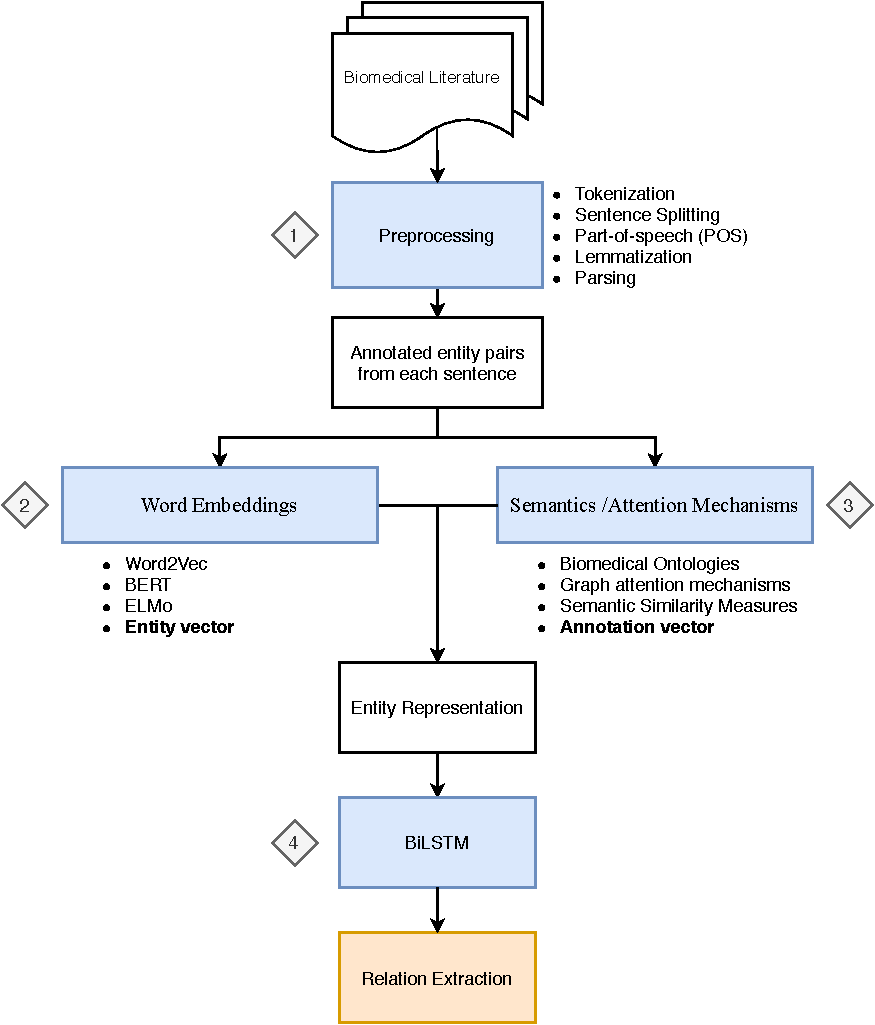
\includegraphics[width=15.5cm]{images/flowchart.pdf}
\caption[Flowchart Illustrating Proposed System]{Flowchart illustrating the proposed deep learning system for biomedical relation extraction combining external sources of knowledge, with the numbered main steps.}
\label{flow}
\end{figure}

\begin{enumerate}
    \item  \textbf{Preprocessing} The preprocessing step will encompass tokenization, sentence splitting, part-of-speech (POS) tagging, lemmatization, and parsing. Each set of biomedical entities has distinct textual characteristics, inherent to unique contexts. Each entity will be identified with a domain-specific Named-Entity Recognition (NER) system \citep{yadav2019survey}. Regarding Named-Entity Linking (NEL), entities such as genes, chemicals, diseases, and proteins, will be matched to an identifier through the corresponding ontology. These tasks need to be optimized to perform RE.   
    \item \textbf{Word Embbeddings} Recurrent Neural Networks (RNN) train classification models based on word embeddings and other features. This system is going to incorporate different state-of-the-art word embeddings like Word2Vec \citep{li2017neural}, ELMo \citep{peters2018deep} and BERT \citep{lin2016neural}, and make use of different combinations of channels to maximize performance.
    \item \textbf{Semantics/Attention Mechanisms} Taking advantage of semantics can provide supplementary information that may not be present in the training data. Ontologies formalize existing knowledge about entities such as genes \citep{ashburner2000gene}, and diseases \citep{schriml2012disease}. Through representation of each entity as the sequence of its ancestors, it is possible to detect new relations between entities that were not evident by only using the training data. Also, a new word embedding layer is going to be built taking advantage of semantics/attention mechanisms. Word embeddings usually represent a variable length sentence into a fixed length vector, where each element of the vector encodes some semantics of the original sentence. The innovation resides in adding the ontology semantics of the identified entity to each vector, as well a graph attention mechanism, and test the use of semantic similarity measures. For example, if the \textit{BRCA1} gene is semantically similar to the \textit{BRAF} gene and the \textit{BRCA1} has an established relation with the \textit{tumor} phenotype, it could be possible to infer that \textit{BRAF} gene also has a relation with the \textit{tumor} phenotype, even if that is not evident by the training data.
    \item \textbf{BiLSTM} The RE system between the linked identified entities is going to be built using bidirectional Long Short-Term Memory (LSTM) networks, a deep learning method that deals with long sentences of words, with a similar architecture to RNN, based on the work of \cite{lamurias2019bo} (BO-LSTM system). These models use different types of information, known as channels, such as word embeddings, part-of-speech tags, grammatical relations, and WordNet hypernyms \citep{ciaramita2006broad}. Each of these channels has different types of input information and is responsible for one of the model layers. All of these layers can be connected to a softmax layer outputting the probabilities of each class. 
\end{enumerate}

\section{Evaluation}

The evaluation of deep learning based systems is done by applying the trained models to a gold standard, manually curated by domain experts and unseen by the information extraction system. To compare results obtained with different datasets or different tools we have three distinct state-of-the-art evaluation metrics: recall, precision, and F-measure.

\begin{enumerate}
    \item Evaluation of the integrated system on different benchmark datasets: The developed systems will use benchmark datasets, such as the semantic relations between pairs of nominals corpus SemEval-2010 Task 8 \citep{hendrickx2010semeval}, the drug-drug interactions corpus SemEval-2013 task-9 \citep{segura2013semeval}, and the Phenotype-Gene Relations corpus \citep{sousa2019silver}.
    \item Development of an improved automated corpus creation based on the PGR corpus for system assessment \citep{sousa2019silver}: Improving automating corpus creation is of interest to create training data for the developed systems since some biomedical relations do not have gold standard corpus available to use to test the quality of these systems. Leveraging on previous work \citep{sousa2019silver} it is possible to generate multiple silver standard corpus for different entities with good enough results. These results have been demonstrated to be sufficient for training deep learning-based systems.
    \item  Application of the systems to other fields and to different languages: Apply domain-specific ontologies of non-biomedical topics, for example, the Planteome, a plant ontology \citep{cooper2018planteome}, using benchmark datasets. Also, making use of the translation of some ontologies like the HPO, and the DECS ontology \citep{campanatti2010health} (i.e., Health Sciences Descriptors in Portuguese and Spanish) linked to English mesh terms \citep{papagiannopoulou2016large}, will allow us to study the effect of different languages in the system.
    \item Participation in different competitions such as SemEval, BioCreative, and BioASQ \citep{huang2016community}.
\end{enumerate}

\section{Case Studies}

The case studies of this project are going to be human phenotypic abnormalities and the identification of cancer-nutrition interactions regarding our collaboration with the World Health Organization (WHO). There is no RE deep learning system that uses the knowledge from the HPO \citep{robinson2010human} to extract relevant clinical information.

Human phenotype terms often have more than one word, are descriptive, and do not follow a specific nomenclature. The individual features of these terms and the subcategory of cancer-related phenotypes will be studied to resolve the preprocessing step and identify the most appropriate semantic additions to the system.  

Through these methods, it will be possible to identify new relation candidates for gold standard knowledge bases of both relations between human phenotype entities and other biomedical entities and cancer-nutrition interactions. Thus, the system will be able to train models using pre-existing datasets to identify new relations between human phenotypes and other biomedical entities and cancer-nutrition interactions.

\section{Planning}

The thesis project encompasses three main objectives, related to deep learning, semantics, and their application to the biomedical domain. Some of the sub-objectives may overlap, and implementation and assessment will continuously incorporate the software developed in the previous steps.

Figure \ref{figure:timeline} presents the timeline of the objectives and sub-objectives of the thesis.

\begin{landscape}

\begin{figure}
\captionsetup{font=small}
\centering
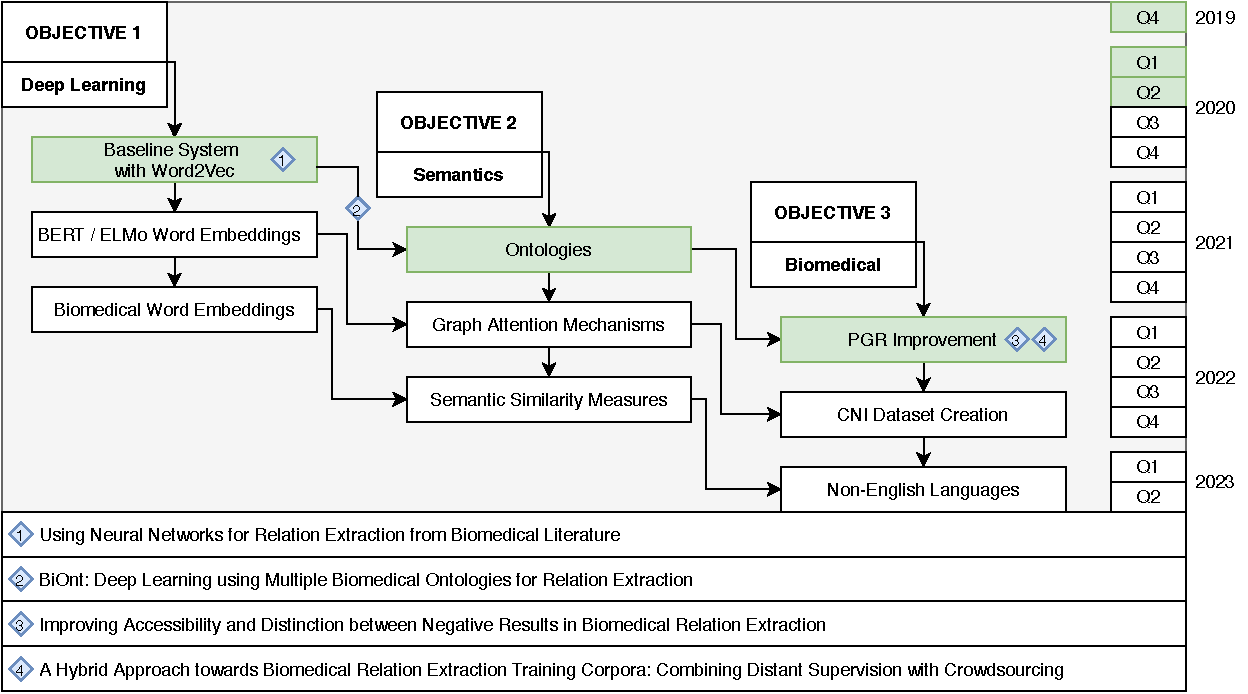
\includegraphics[width=20cm]{images/timeline.pdf}
\fontsize{9}{10.8}\caption[Thesis Project Timeline]{Project timeline. Main objectives and sub-objectives of the thesis. In green, the sub-objectives already fulfilled (according to the timeline). Identified with 1, 2, 3, and 4 are the articles published (1-3) and submitted (4) and to what thesis step they refer. PGR stands for the Phenotype-Gene Relations dataset and CNI for cancer-nutrition interactions.}
\label{figure:timeline}
\end{figure}

\end{landscape}